\documentclass{standalone}
\usepackage{tikz}
\usetikzlibrary{angles, quotes}

\begin{document}

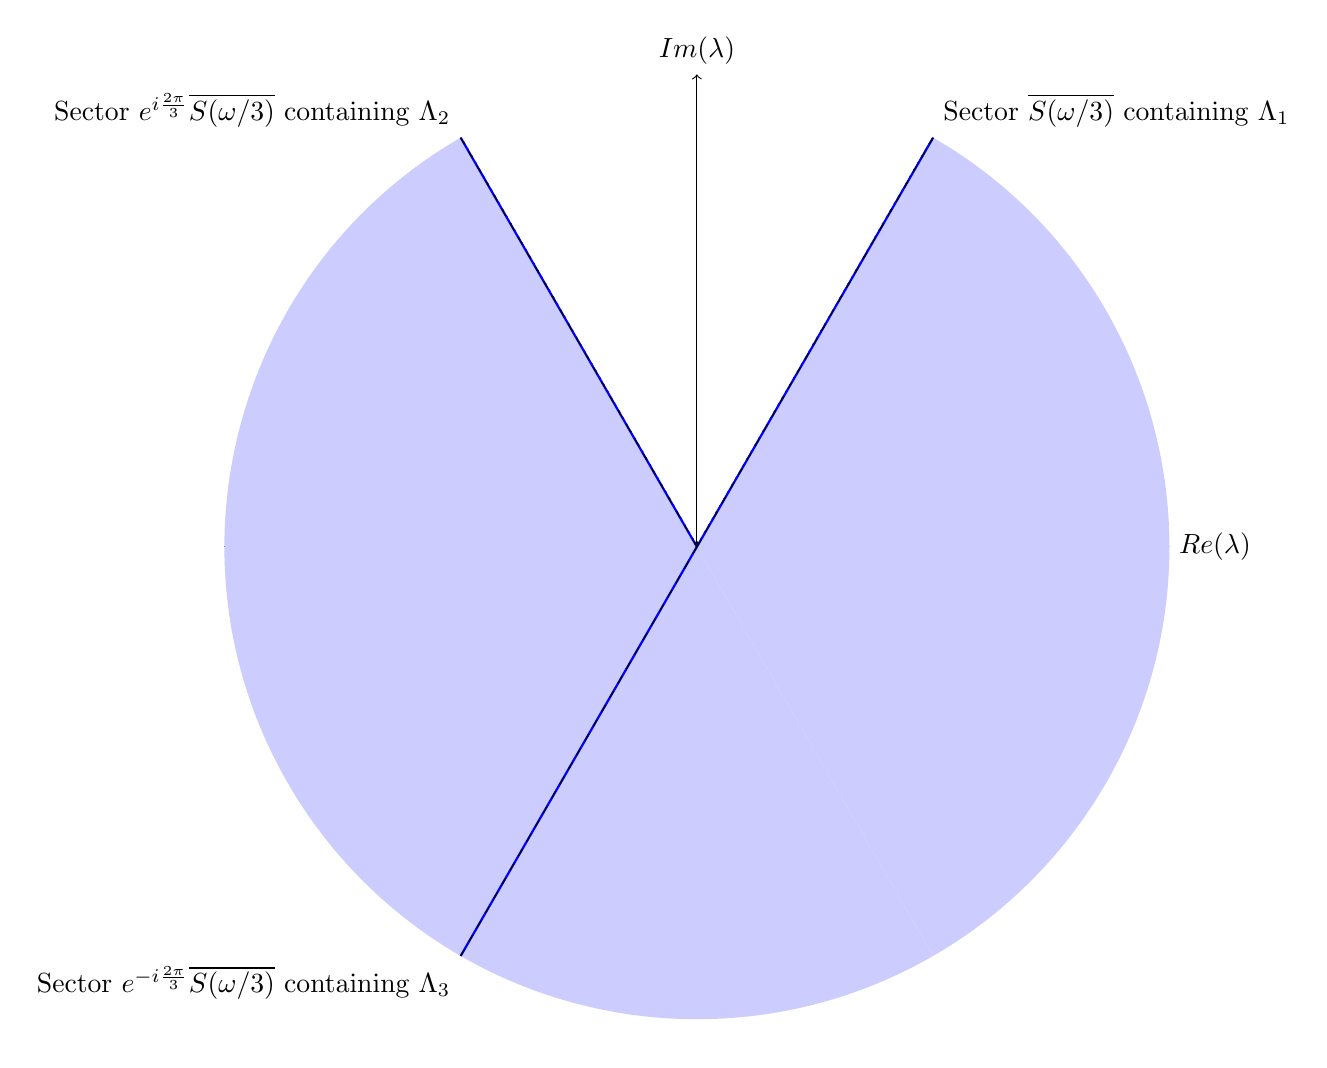
\begin{tikzpicture}[scale=2]
    % Axes
    \draw[->] (-3,0) -- (3,0) node[right] {$\operatorname{Re}(\lambda)$};
    \draw[->] (0,-3) -- (0,3) node[above] {$\operatorname{Im}(\lambda)$};

    % Origin
    \fill (0,0) circle (1pt);

    % Label for omega
    \node at (1.5,0) {$\omega$};

    % Sectors
    \draw[dotted, thick] (0,0) -- (60:3) node[above right] {Sector $\overline{S(\omega/3)}$ containing $\Lambda_1$};
    \draw[dotted, thick] (0,0) -- (240:3) node[below left] {Sector $e^{-i\frac{2\pi}{3}}\overline{S(\omega/3)}$ containing $\Lambda_3$};
    \draw[dotted, thick] (0,0) -- (120:3) node[above left] {Sector $e^{i\frac{2\pi}{3}}\overline{S(\omega/3)}$ containing $\Lambda_2$};

    % Fill sectors
    \fill[blue!20] (0,0) -- (60:3) arc (60:-60:3) -- cycle;
    \fill[blue!20] (0,0) -- (240:3) arc (240:300:3) -- cycle;
    \fill[blue!20] (0,0) -- (120:3) arc (120:240:3) -- cycle;

    % Blue lines
    \draw[thick, blue] (0,0) -- (60:3);
    \draw[thick, blue] (0,0) -- (120:3);
    \draw[thick, blue] (0,0) -- (240:3);

    % Dashed lines
    \draw[dashed] (0,0) -- (60:3);
    \draw[dashed] (0,0) -- (120:3);
    \draw[dashed] (0,0) -- (240:3);

\end{tikzpicture}

\end{document}